\documentclass[fleqn]{article}

\usepackage{graphicx}
\usepackage{xurl}
\usepackage{url}
\usepackage{caption}
\usepackage{fancyhdr}
\usepackage{mathtools}
\usepackage{amsmath}
\usepackage{amssymb}
\usepackage{tikz}
\usepackage{listings}
\usepackage{xcolor}
\usepackage{float}

\definecolor{codegreen}{rgb}{0,0.6,0}
\definecolor{codegray}{rgb}{0.5,0.5,0.5}
\definecolor{codepurple}{rgb}{0.58,0,0.82}
\definecolor{backcolour}{rgb}{0.95,0.95,0.92}

\lstdefinestyle{mystyle}{
    backgroundcolor=\color{backcolour},   
    commentstyle=\color{codegreen},
    keywordstyle=\color{magenta},
    numberstyle=\tiny\color{codegray},
    stringstyle=\color{codepurple},
    basicstyle=\ttfamily\footnotesize,
    breakatwhitespace=false,         
    breaklines=true,                 
    captionpos=b,                    
    keepspaces=true,                 
    numbers=left,                    
    numbersep=5pt,                  
    showspaces=false,                
    showstringspaces=false,
    showtabs=false,                  
    tabsize=2
}

\lstset{style=mystyle}

\usepackage{xepersian}

\settextfont[BoldFont={XB Zar bold.ttf}]{XB Zar.ttf}
\setlength\parindent{0pt}



\newcommand{\expnumber}{دوم}



\title{

\includegraphics[width=0.4\textwidth]{sharif.png}\\
\normalsize{دانشکده مهندسی کامپیوتر}\\
\vspace{1cm}
    
\huge{آزمایشگاه معماری کامپیوتر}
\\ \vspace{.8cm}
\Large{گزارش آزمایش \expnumber}
\\ \vspace{.8cm}
\Large{عنوان آزمایش : ضرب‌کننده ممیز ثابت}
}

\author{
\\
دکتر حمید سربازی آزاد
\\ \vspace{.4cm}
\\
  سارا آذرنوش       ---      98170668
\\ \vspace{0.2cm} \\
  کسری امانی       ---      98101171
\\ \vspace{0.2cm} \\
  پارسا محمدیان       ---      98102284
\\ \vspace{.4cm}
}

\date{\today}

\begin{document}

\clearpage\maketitle
\thispagestyle{empty}

\newpage

\pagestyle{fancy}
\lhead{آزمایشگاه معماری کامپیوتر}

\rhead{آزمایش \expnumber}

\tableofcontents

\setcounter{page}{1}

\newpage

\section{مقدمه}
در این آزمایش باید یک ضرب‌کننده با روش 
\lr{Shift and Add} 
طراحی کنیم. مدرا ضرب‌کننده یک مدار ترتیبی است. که از یک جمع‌کننده و چند ثبات با قابلیت شیفت 
و یک واحد کنترل تشکیل شده است.

\section{هدف آزمایش}
طراحی مدار ترتیبی ضرب‌کننده 4 بیت در 4 بیت با نرم‌افزار پروتئوس.

\section{شرح آزمایش}
برای طراحی چنین مداری ابتدا رفتار آن را با نمودار 
\lr{ASM} 
مشخص می‌کنیم. نمودار 
\lr{ASM} 
در شکل 
\ref{asm}
آمده است.

\begin{figure}[!htbp]
    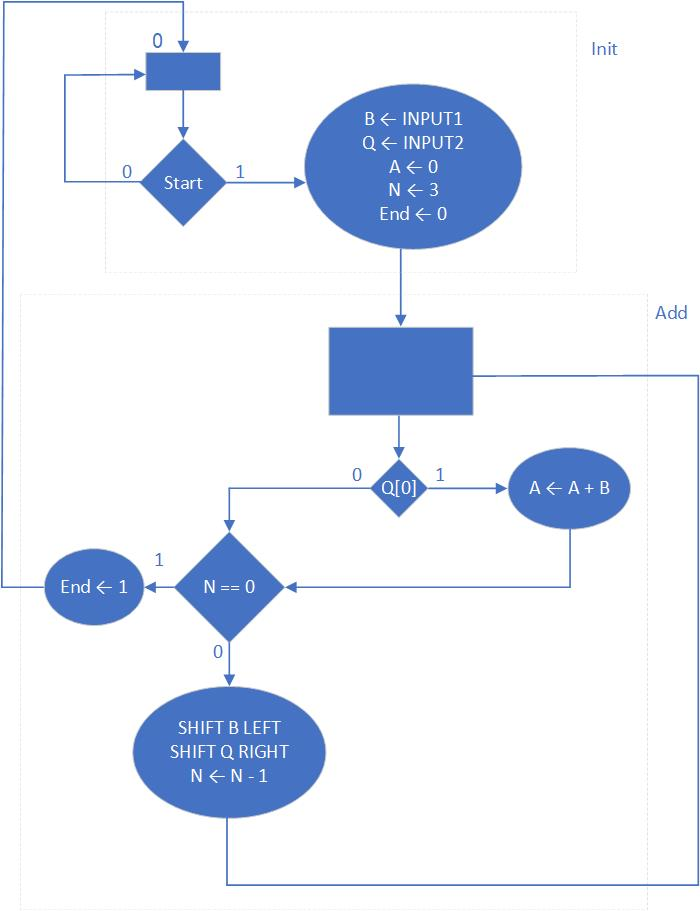
\includegraphics[width=\textwidth]{Assets/asm.jpg}
    \caption{نمودار \lr{ASM}}
    \label{asm}
\end{figure}

سه رجیستر داریم که مقادیر ضرب شونده، ضرب کننده و حاصل ضرب در آن‌ها هستند. 
با توجه به الگوریتم 
\lr{Shift and Add}
،مدار به صورت زیر طراحی میشود:
مضروب فیه به راست شیفت میخورد و در صورتی که اولین رقم آن از راست 1 باشد جمع میکند.
مقدار ضرب شونده در یک رجیستر قرار دارد که به چپ شیفت میخورد و مقدار آن با مقدار حاصل جمع میشود
رجیستر حاوی حاصل ضرب در صورتی که مقدار مضروب فیه یک باشد مقدار حاصل جمع را لود میکند.
تعداد شیفت ها به اندازه تعداد بییت‌ها 4 است که 
با استفاده از کانتر و فلیپ فلاپ استیت کنترل میشود در صورتی که 4 شود عملیات ضرب پایان میابد.

مدار استیت که شامل فلیپ فلاپ و دو بافر 3 حالته است نیز از روی نمودار حالت رسم شده از 
\lr{ASM}
بدست آمده است که این نمودار حالت در شکل 
\ref{state}
قابل مشاهده است. 

\begin{figure}[!htbp]
    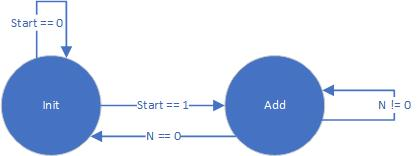
\includegraphics[width=\textwidth]{Assets/state.jpg}
    \caption{نمودار حالت برای کنترل وضعیت‌ها}
    \label{state}
\end{figure}

مدار نهایی در شکل 
\ref{main}
قابل مشاهده است.

\begin{figure}[!htbp]
    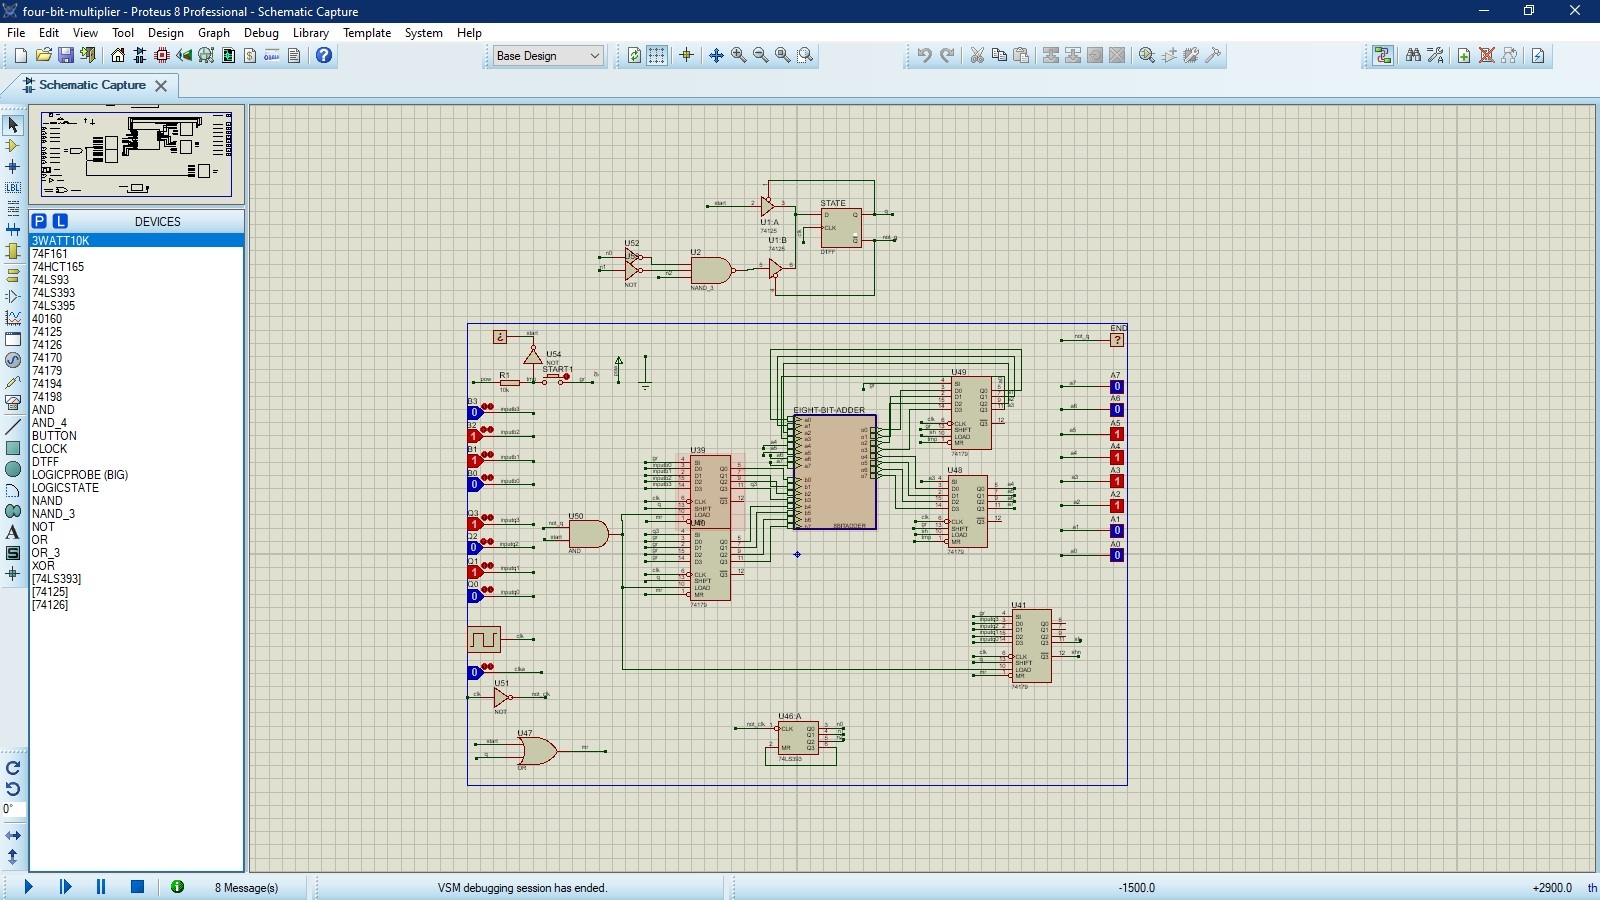
\includegraphics[width=\textwidth]{Assets/maincirc.jpg}
    \caption{مدار نهایی}
    \label{main}
\end{figure}

\section{نتیجه آزمایش}
یک ضرب کننده 4 بیت در 4 بیت داریم که با استارت شروع به کار میکند و هنگامی که end 
یک میشود حاصل آماده است. دقت شود که کلید استارت باید انقد نگه داشته شود تا سیگنال 
\lr{End}
صفر شود سپس کلید رها شود و عملیات ضرب شروع می‌شود.

مدار را به ازای ورودی‌های مختلف تست می‌کنیم. شاهد هستیم حاصل ضرب دو عدد 14 و 9 در شکل 
\ref{test1}
به درستی محاسبه شده است. 

در کشل 
\ref{test2}
هم حاصل ضرب 6 و 10 نیز به درستی محاسبه شده است.

\begin{figure}[!htbp]
    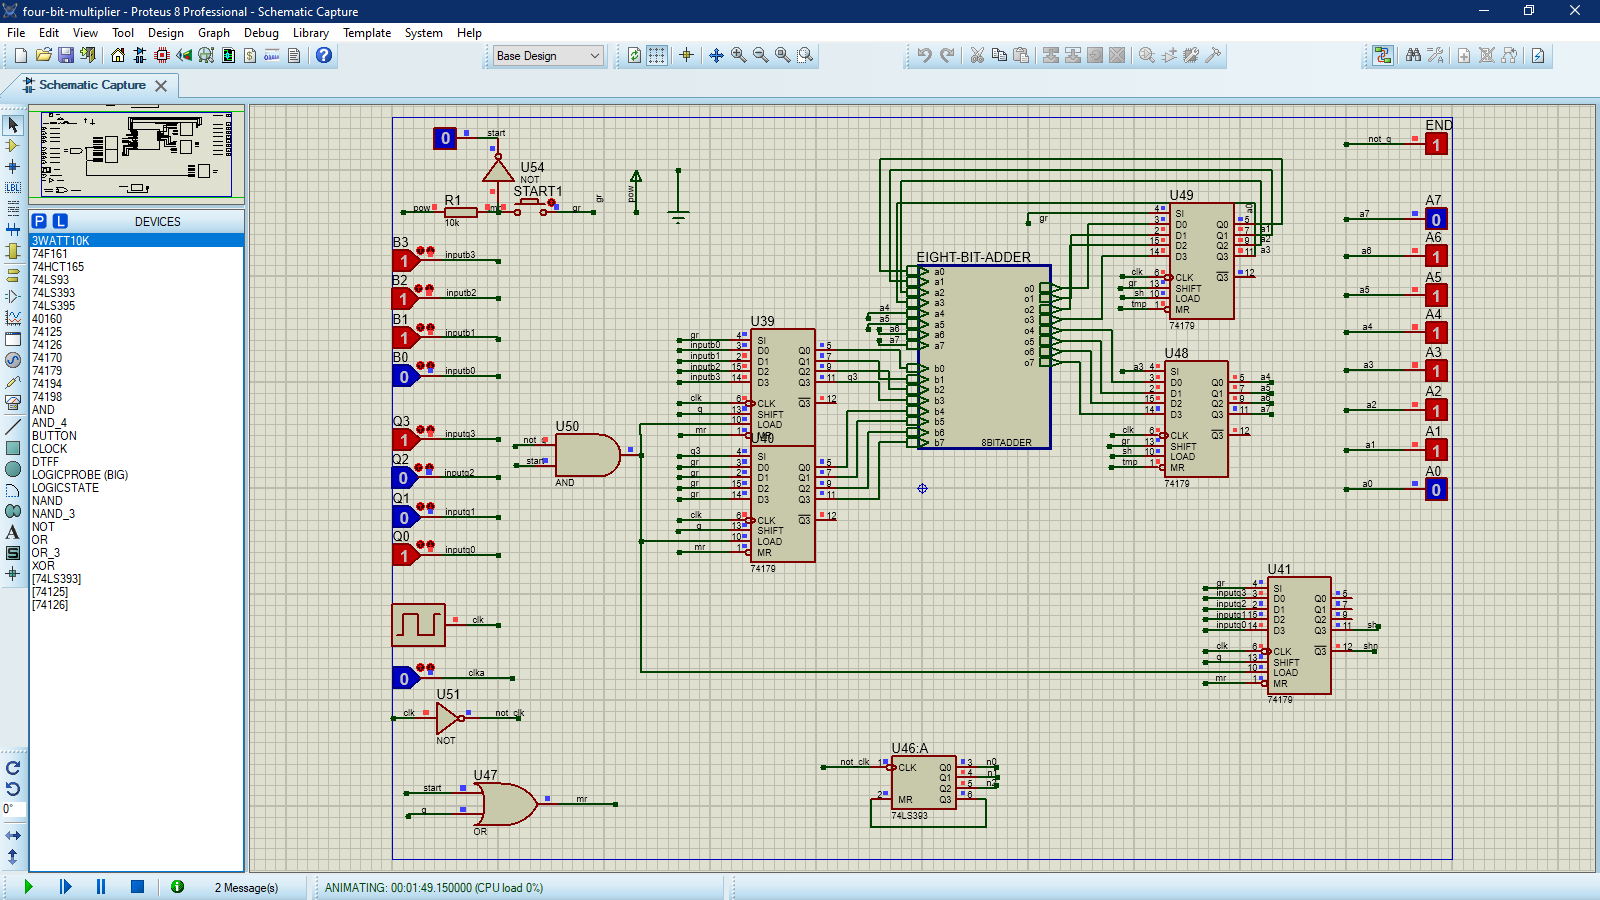
\includegraphics[width=\textwidth]{Assets/test1.jpg}
    \caption{تست 1}
    \label{test1}
\end{figure}

\begin{figure}[!htbp]
    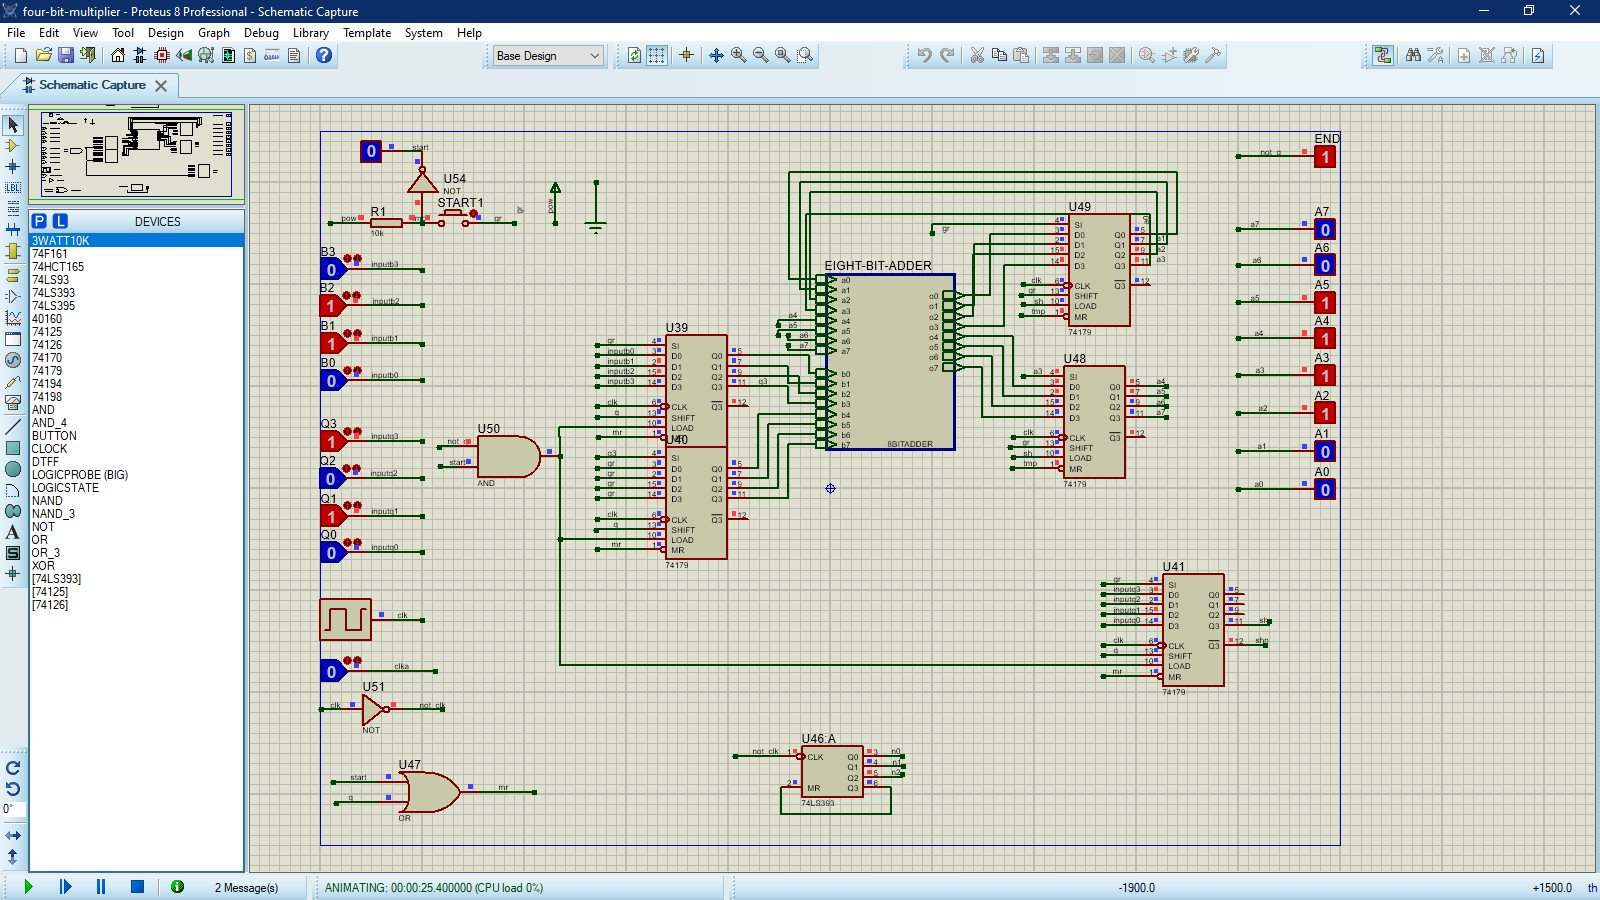
\includegraphics[width=\textwidth]{Assets/test2.jpg}
    \caption{تست 2}
    \label{test2}
\end{figure}

\end{document}